\chapter{Modern Biological Data Management and Analysis}\label{biodata}
From the discovery of the \gls{dna} structure by Watson and Crick in
1953\cite{watson1953molecular} to the sequencing of the human genome in
2001,\cite{venter2001sequence,international2001initial} and the massively
parallel sequencing platforms in the later years\cite{metzker2010sequencing},
the scientific advances have been tremendous. Today, single week-long sequencing
runs can produce as much data as did entire genome centers just years
ago.\cite{kahn2011future}  These technologies allow researchers to produce data
faster, cheaper and more efficiently, now making it possible to sequence the
entire genome from a patient in less than a day. In addition to faster
data generation, the new datasets are also of higher quality.

Ensuring reproducibility through sharing of analysis code and datasets is
necessary to advance science.\cite{baker2016scientists} From the many obstacles
to replicate results from the most influential papers in cancer
research\cite{reprod}, it is apparent that it is important to thoroughly
document the entire workflow from data collection to interpretable results.
This requires implementing best practices for data storage and processing. Such
best practices are also necessary for large and complex research studies where
data collection, analysis, and interpretation may span decades, and therefore be
done in several iterations. 

In this chapter we describe our efforts to establish an approach for
reproducible analysis of biological data in a complex epidemiological study. We
first give a short introduction to high-throughput datasets, before describing
the \gls{nowac} study we have used as a motivating example. We describe the
previous practice for data management and analysis, and propose a new approach
to achieve reproducible analyses. Continuing, we show that our approach to
manage research data and code can be used to develop a standardized data
analysis pipeline. Further we provide best practices for data analysis and
management. 

\section{High-Throughput Datasets for Research and Clinical Use} 
High-throughput technologies that are now widely used to study complex diseases
such as cancer. \gls{dna} sequencing is the process of determining the order of
nucleotides within a strand of \gls{dna}. \gls{hts}, or \gls{ngs}, is a term
used to describe newer technology that enables massively-parallel sequencing of
\gls{dna}. \gls{hts} instruments sequence millions of short base pairs, and we
assemble these in the data analysis process. Typical sequencing datasets are in
the size of hundreds of \glspl{gb} per sample. 

While \gls{hts} can study the sequence of bases, microarrays have been used to
study the transcriptome, or the genes actively expressed. While the genome is
mostly fixed for an organism, the transcriptome is continuously changing. These
instruments report the expression levels of many target genes, and
by profiling these we can study which genes are active in the biological sample.
Microarray datasets are in the size of megabytes per sample. 

Another technique to study the transcriptome is to use \gls{rna}-seq technology
based on \gls{hts}. \gls{rna}-seq instruments also read millions of short base
pairs in parallel, and can be used in gene expression analysis. Because of its
higher quality output, \gls{rna}-seq is the successor to microarray technology.
These datasets are also in the size of hundreds of \glspl{gb}.

Precision medicine uses patient-specific molecular information to diagnose and
categorize disease to tailor treatment to improve health
outcome.\cite{national2011toward} Important research goal in precision medicine
are to learn about the variability of the molecular characteristics of
individual tumors, their relationship to outcome, and to improve diagnosis and
therapy.\cite{tannock2016limits} International cancer institutions are therefore
offering dedicated personalized medicine programs, but while the data collection
and analysis technology is emerging, there are still unsolved problems to enable
reproducible analyses in clinical settings. For cancer, \gls{hts}
is the main technology to facilitate personalized diagnosis and
treatment, since it enables collecting high quality genomic data from patients
at a low cost. 

\section{Norwegian Women and Cancer (\gls{nowac})}
In this thesis we have used data from the \gls{nowac} study extensively. 
The \gls{nowac} study is a prospective population-based cohort that tracks 34\%
(170.000) of all Norwegian women born between 1943–57.\cite{nowac} The data
collection started in \gls{nowac} in 1991 with surveys to cover, among others,
the use of oral contraceptives and hormonal replacement therapy, reproductive
history, smoking, physical activity, breast cancer, and breast cancer in the
family. The datasets are also integrated with data from The Norwegian Cancer
Registry, and The Cause of Death Registry in Statistics Norway. In addition
to the questionnaire data, the study includes blood samples from 50.000 women,
as well as more than 300 biopsies. From the biological samples the first gene
expression dataset was generated in 2009, and the study now also features miRNA,
methylation, metabolomics, and \gls{rna}-seq datasets. 

The data in the \gls{nowac} cohort allows for a number of different study
designs. While it is a prospective cohort study, we can also draw a case-control
study from the cohort, or a cross-section study from the cohort. From the
\gls{nowac} cohort there has been published a number of research papers that
investigate the questionnaire data together with the gene expression
datasets.\cite{olsen2013plasma,dumeaux2010deciphering}  We have also used the
gene expression datasets to explore gene expression signals in blood and
interactions between the tumor and the blood systemic response of breast cancer
patients.\cite{holden2017local, dumeaux2017interactions}. Some analyses have
resulted in patents\cite{blobrec} and commercialization efforts.  While many
interesting patterns and results have been studied, there are still many
unexplored areas in the available datasets.

In the \gls{nowac} study we are a traditional group of researchers, PhD and
Post-Doc students, and administrative and technical staff. Researchers have
backgrounds from statistics, medicine, or epidemiology, and now also computer
science. The administrative and technical staff is responsible for managing the
data, both data collection and data delivery to researchers. 

\subsection{Data Management and Analysis} 
Surveys are the traditional data collection method in epidemiology. But
today, questionnaire responses are increasingly integrated with molecular data.
However, surveys are still important for designing a study that can answer
particular research questions.  In this section we describe how such integrated
data analysis was done in \gls{nowac} before we developed our approach. We
believe many studies have, or are still, analyzing epidemiological data using
a similar practice. 

In the \gls{nowac} study we have stored the raw survey and registry data in an
in-house database backed up to an independent storage node. Previously,
researchers had to apply to get data exported from the database by an engineer.
This was typically done through SAS scripts that did some preprocessing, e.g.
selecting applicable variables or samples, before the data was sent to
researchers as SAS data files. The downstream analysis was typically done in
SAS. Researchers used e-mail to communicate and send data analysis scripts, so
there was not a central hub with all the scripts and data. 

In addition to the questionnaire data, the \gls{nowac} study also integrates
with registries which are updated regularly. The datasets from the different
registries are typically delivered as \gls{csv} files to our scientific staff,
which are then processed into a standardized format. Since the \gls{nowac} study
is a prospective cohort, a percentage of the women are expected to get a cancer
and move from the list of controls into the list of cases. 

In the \gls{nowac} study we have processed our biological samples outside our
research institution. The received raw datasets were then stored on a
local server and made available to researchers on demand. Because of the
complexity of the biological datasets, many of these require extensive
pre-processing before they are analysis-ready. 

% \section{Reproducible Research} 

\section{Enabling Reproducible Research} 
To enable reproducible research in the \gls{nowac} study we have developed a
system for managing and documenting the available datasets, a standardized data
preprocessing and preparation system, and a set of best practices for data
analysis and management. We designed our management and analysis system as a
\gls{sme} that we could later use in the Pippeline system. To determine the
demands of the users, we collaboratively identified issues with our previous
practice and a set of requirements for a system to solve these issues.

We first identified issues with our previous practice: 
\begin{enumerate} 
    \item It was difficult to keep track of the available datasets, and to
        determine how these had been processed. We had no standard data storage
        platform or structure, and there were limited reports for exported
        datasets used in different research projects.
        
    \item There was no standard approach to preprocess and initiate data
        analysis. This was because the different datasets were analyzed by
        different researchers, and there was little practice for sharing
        reusable code between projects. 

    \item It became difficult to reproduce the results reported in our published
        research manuscripts. This was because the lack of standardized
        preprocessing, sharing of analysis tools, and full documentation of the
        analysis process. 
        
\end{enumerate} 

To solve these issues and enable reproducible research in the \gls{nowac} study,
we had to develop a system for managing the data, code, and our proposed best
practices for analyzing the data. We started with identifying a set of
requirements for a system to manage and document the different datasets: 

\begin{itemize} 
    \item It should provide users with a single interface to access the
        datasets, their respective documentation, and utility functions to
        access and analyze the data.
    \item It should provide version history for the data and analysis code. 
    \item The system should provide reproducible data analysis
        reports\footnote{Such as an R Markdown file which, when executed,
        generates the output data and optional documentation including plots,
        tables etc.} for any dataset that has been modified in any way. 
    \item It should be portable and reusable by other systems or applications. 
\end{itemize} 

To satisfy the above requirements we developed the \texttt{nowac} R package, a
software package in the R programming language that provides access to all data,
documentation, and utility functions. Since it is a requirement that it should
be reusable we could then implement a data preparation system, Pippeline, ontop
of this R package. We identified a set of requirements for this data
preprocessing and preparation system as well: 

\begin{itemize} 
    \item The data preprocessing and preparation system should provide users
        with an interactive point-and-click interface to generate anlaysis-ready
        datasets from the \gls{nowac} study. 
    \item It should use the \texttt{nowac} R package to retrieve datasets. 
    \item It should provide users with a list of possible options for filtering,
        normalization, and other options required to preprocess a microarray
        dataset.
    \item It should genererate a reproducible report along with any exported
        dataset.
\end{itemize} 

Finally, we developed a set of best practices for data analysis in our study. In
the rest of the section we detail how we built the \texttt{nowac} package, the
Pippeline, and the best practices for data analysis. 

\subsection{The \texttt{nowac} Package} 
The \texttt{nowac} R package is our solution for storing, documenting, and
providing analyis functions to process the datasets in the \gls{nowac} study. We
use \texttt{git} to version control the analysis code and datasets, and store
the repository on a self-hosted git server.  We bundle together all datasets in
the \texttt{nowac} package. This includes both questionnaire, registry, and gene
expression datasets. Because none of these are particularly large (no single
dataset being more than tens of \glspl{gb}) we are able to distribute them with
our R package. Some datasets require pre-processing steps such as outlier
removal before the analysts can explore the datasets. For these datasets we
store the \emph{raw} datasets, processed data, and the analysis-ready clean
datasets. We store the raw datasets in their original format, while clean and
processed datasets are stored as R data files to simplify importing them in R.
In addition to the datasets themselves we store the R code we used to generate
the datasets.  For clarity, we decorate the scripts with specially formatted
comments that can be used with knitr\cite{xie2016dynamic} to generate
reproducible data analysis reports. These highlight the transformation of the
data from raw to clean, with information such as removed samples or data
normalization methods. 

We have documented every dataset in R package. The documentation includes
information such as data collection date, instrument types, the persons involved
with data collection and analysis, pre-processing methods etc.  When users
install the \texttt{nowac} package the documentation is used to generate
interactive help pages which they can browse in R, either through a command line
or through an \gls{ide} such as RStudio.  We can also export this documentation
to a range of different formats, and researchers can also view them in the R
interface. Figure \ref{rpkgfig} shows the user interface of RStudio where the
user has opened the documentation page for one of the gene expression dataset. 

In the \gls{nowac} package we also provide utility functions to get started with
the analysis of our datasets. Because of the specialized nature of the different
research project the \gls{nowac} package only contains helper functions to start
analyzing \gls{nowac} data, e.g. retrieving questionnaire data. 

We use a single repository for the R package, but have opted to use \texttt{git
submodules} for datasets in the R package.  This allows us to separate the
access to the datasets, and the documentation and analysis code. Everyone with
access to the repository can view the documentation and analysis code, but only
scientific staff have access to the data.  There are however drawbacks to
creating one large repository for both data and code. Since git stores every
version of a file, these types of repositories may become large if the datasets
are changing a lot over time, and are stored in binary formats, e.g. gene
expression datasets. We have explored different techniques to minimize our
repository and have opted to store all datasets as git
submodules\cite{submodule}. Submodules allow us to keep the main repository size
down while still versioning the data.  There are extensions to git for
versioning large datasets. git-raw\cite{gitraw}, git-annex\cite{gitannex}
git-lfs\cite{gitlfs} all provide extensions that essentially replace 
large files in a git repository with pointers or other metadata, and store the
actual files in an external storage server. Since our datasets are relatively
small and static, we did not opt for any of these. Future versions may
investigating these extensions, but the key point is to version all datasets
using a familiar tool, namely git. 

\begin{figure}
  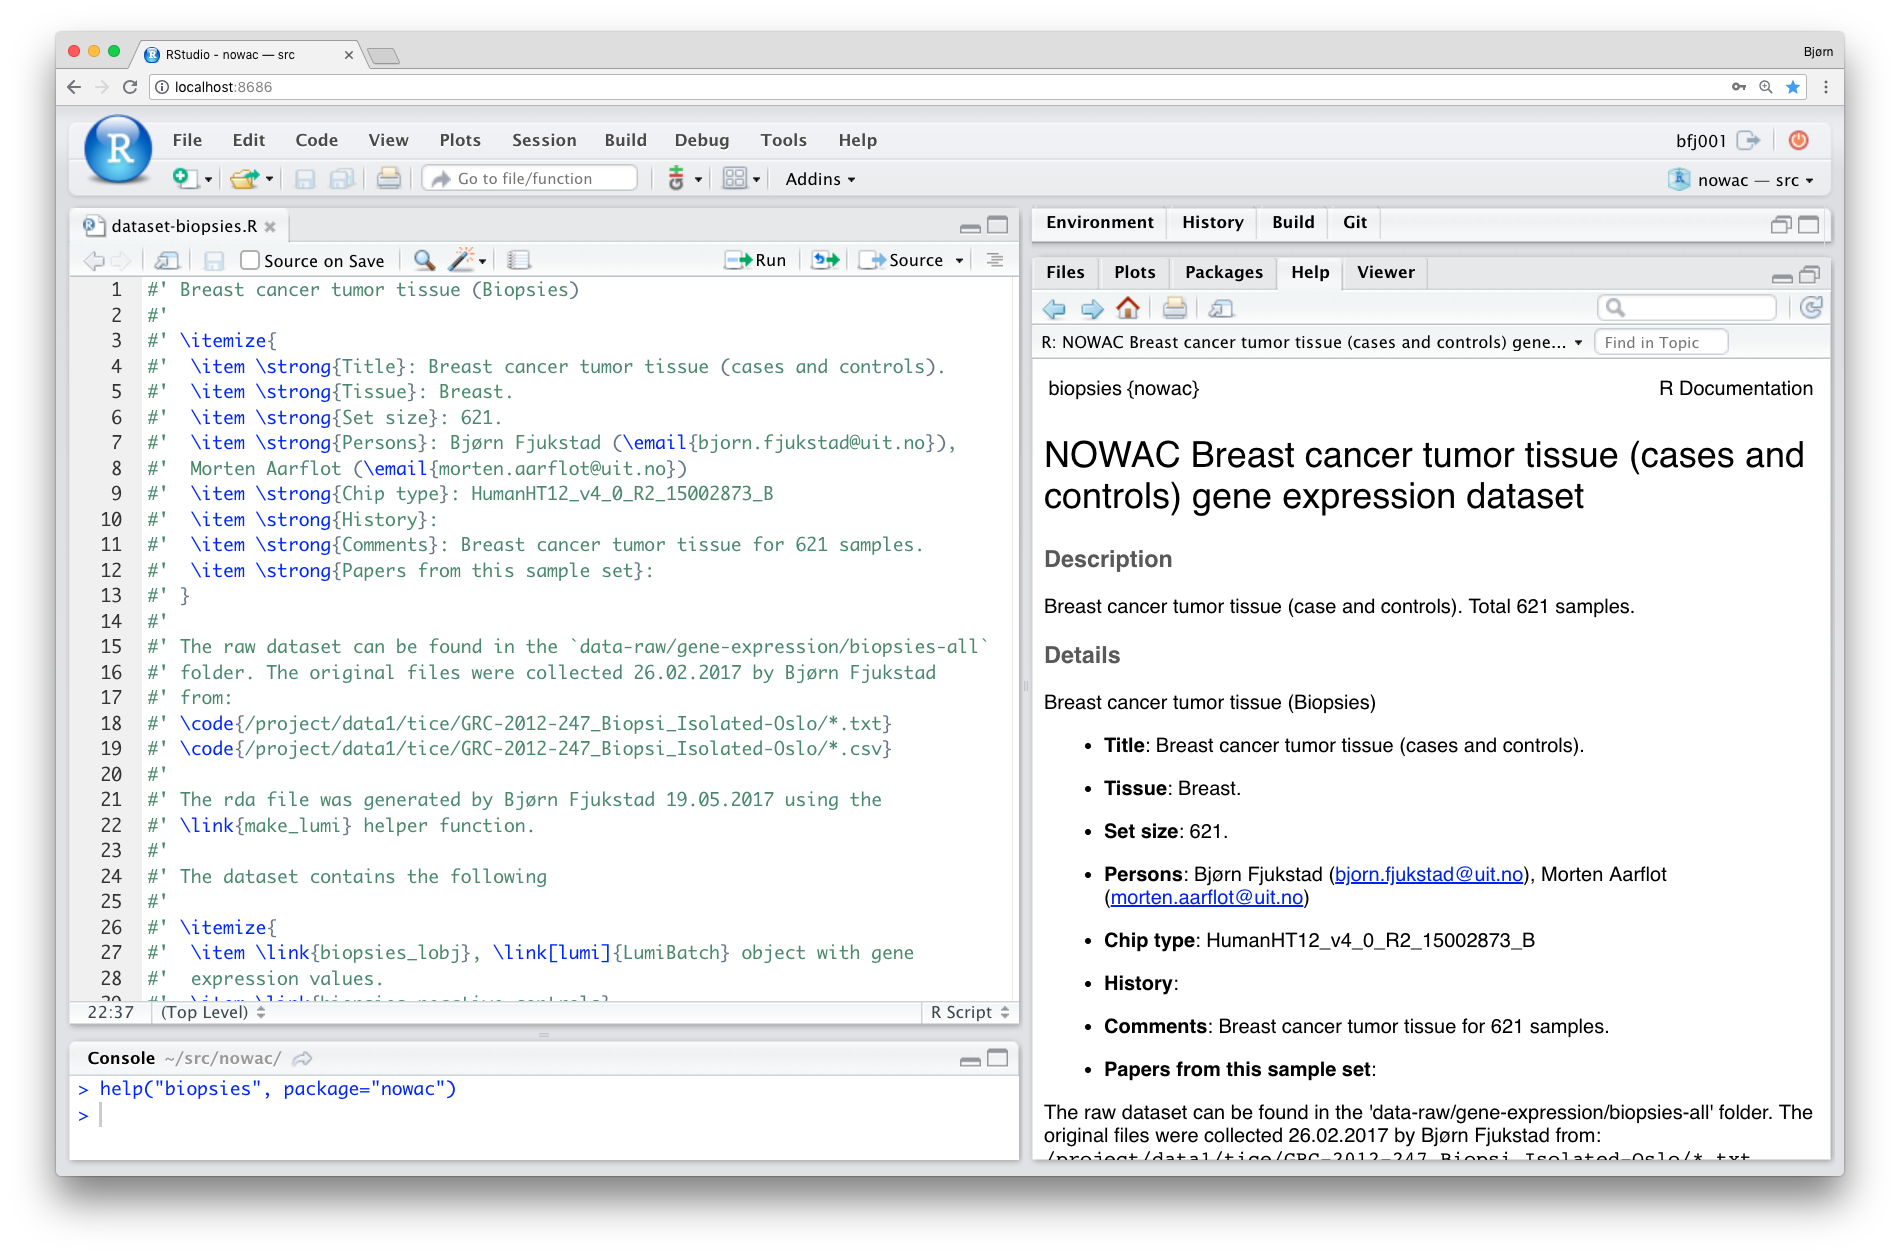
\includegraphics[width=\linewidth]{figures/rpkg.png}
    \caption[A screenshot of the user interface of R Studio.]{A screenshot of
    the user interface of R Studio viewing the documentation help page for the
    "Biopsies" dataset in the \gls{nowac} study.  The right-hand panel shows the
    documentation generated by the code in the top left panel. The bottom left
    panel shows the R command that brought up the help page.}
    \label{rpkgfig} 
\end{figure}

\section{Standardized Data Analysis}
Analyzing the biological data in the \gls{nowac} study consists of four major
parts as show on Figure \ref{fig:uit_pippeline}. First, as explained above the
raw datasets are added to the \texttt{nowac} R package and documented thoroughly
by a data manager.  Second, we manually examine the biological datasets to
detect outliers. We add information about outliers to the \texttt{nowac} R
package along with reports that describe why an observation is marked as an
outlier.  Third, the data manager generates an analysis-ready dataset for a
research project using the interactive Pippeline tool. This dataset is
preprocessed, and integrated with questionnaire and registry datasets. Fourth,
researchers analyze the dataset with their tools of choice, but following
our best practices for data analysis.

\begin{figure}
    \centering
    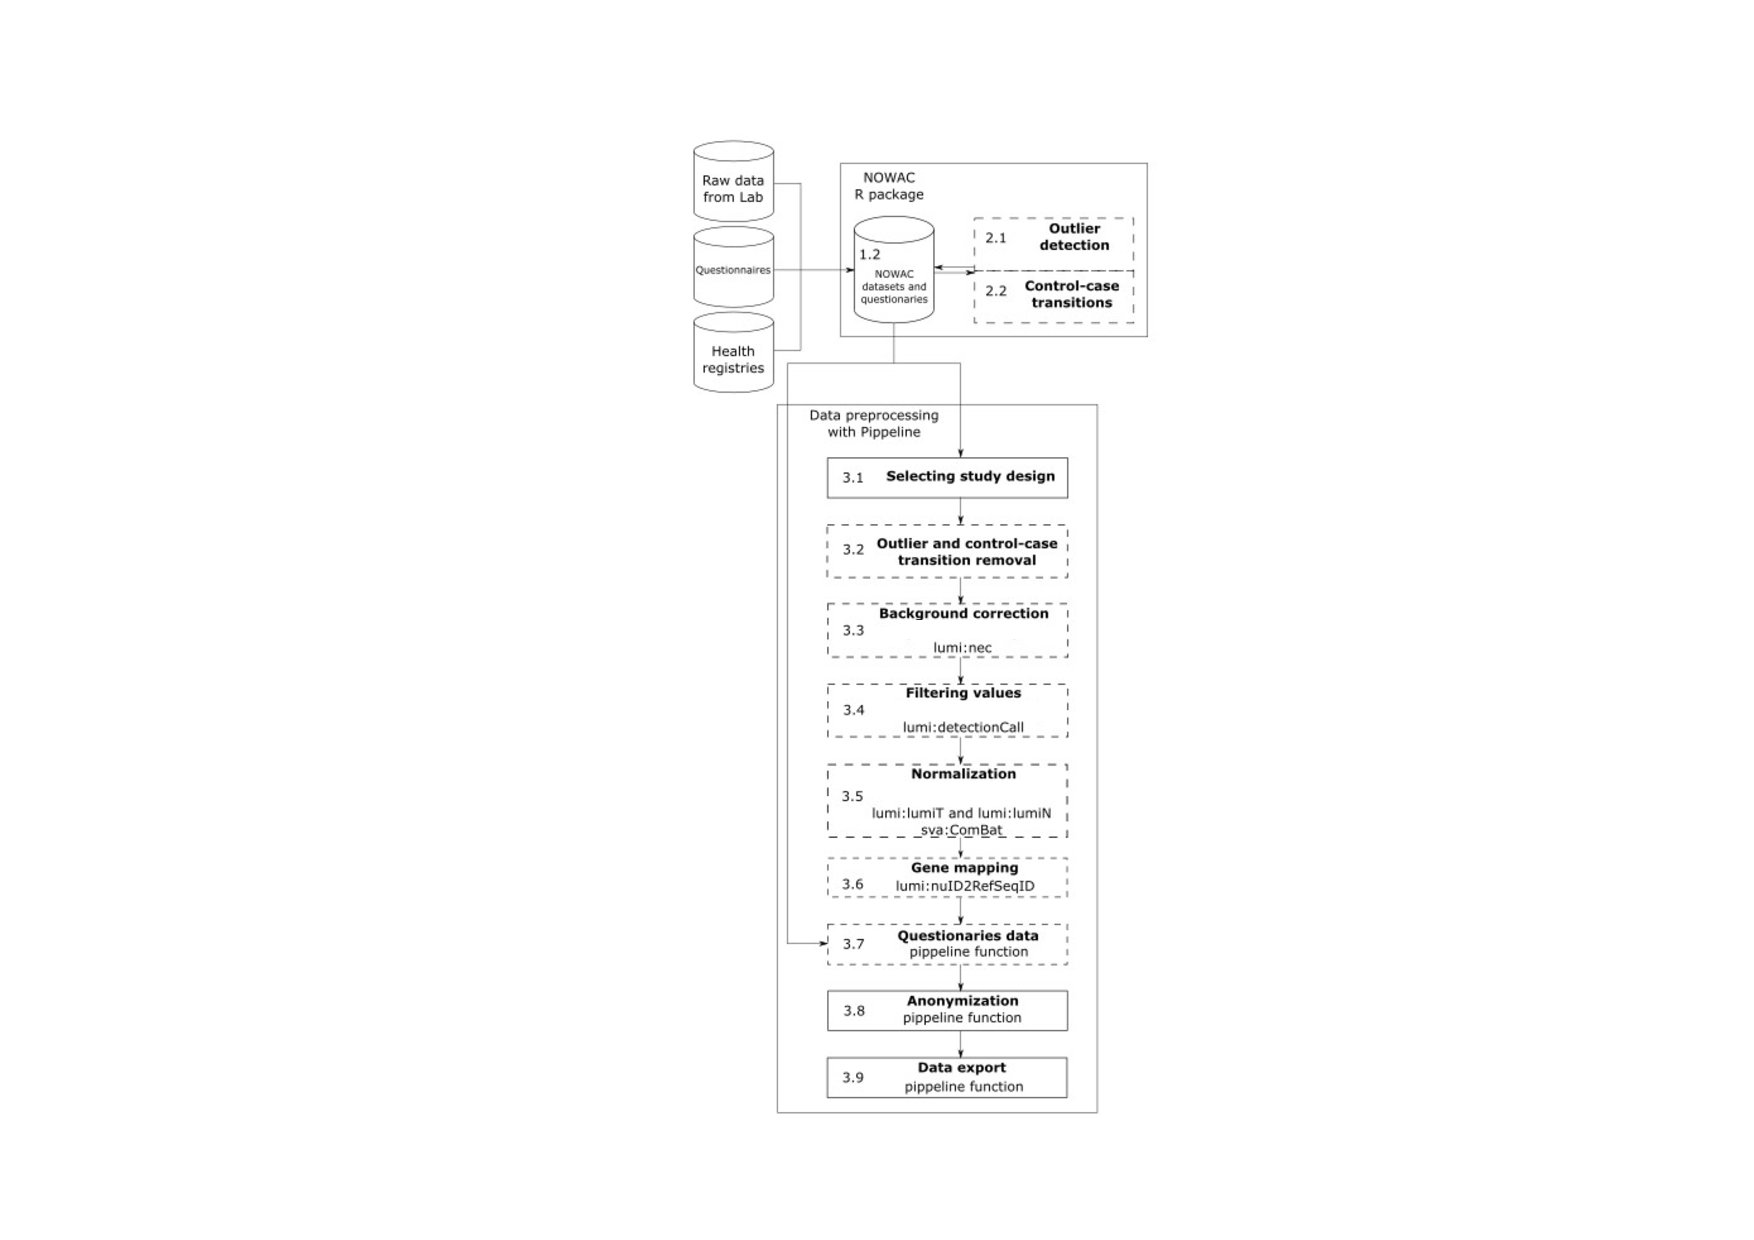
\includegraphics[width=10cm]{figures/uit_pippeline_rm_refs.pdf}
    \caption[Standardized data processing pipeline]{The standardized data
    processing pipeline for gene expression data analysis in the \gls{nowac}
    study. Steps with a dashed line are optional, while steps marked with a
    solid line are mandatory.}
    \label{fig:uit_pippeline}
\end{figure}


\subsection{Pippeline} 
We have developed our preprocessing pipeline for gene expression data as a
point-and-click web application called Pippeline. The web application is
stand-alone and does not require the users to use any command-line tools or have
any programming knowledge. Pippeline generates an analysis-ready dataset by
integrating biological datasets together with questionnaire and registry data,
all found in our \texttt{nowac} package. It uses pre-discovered outliers to
exclude samples, and presents the user with a list of possible processing
options. It exports the analysis-ready R data files together with a reproducible
data analysis report, an R script, that describes all processing steps.  Figure
\ref{fig:scr_filtering} shows the filtering step in Pippeline where users define
at what level they wish to exclude gene expression probes in the dataset. 

The web application is implemented in R using the \texttt{Shiny} framework. It
uses the \texttt{nowac} R package to retrieve all datasets. 

\begin{figure}
    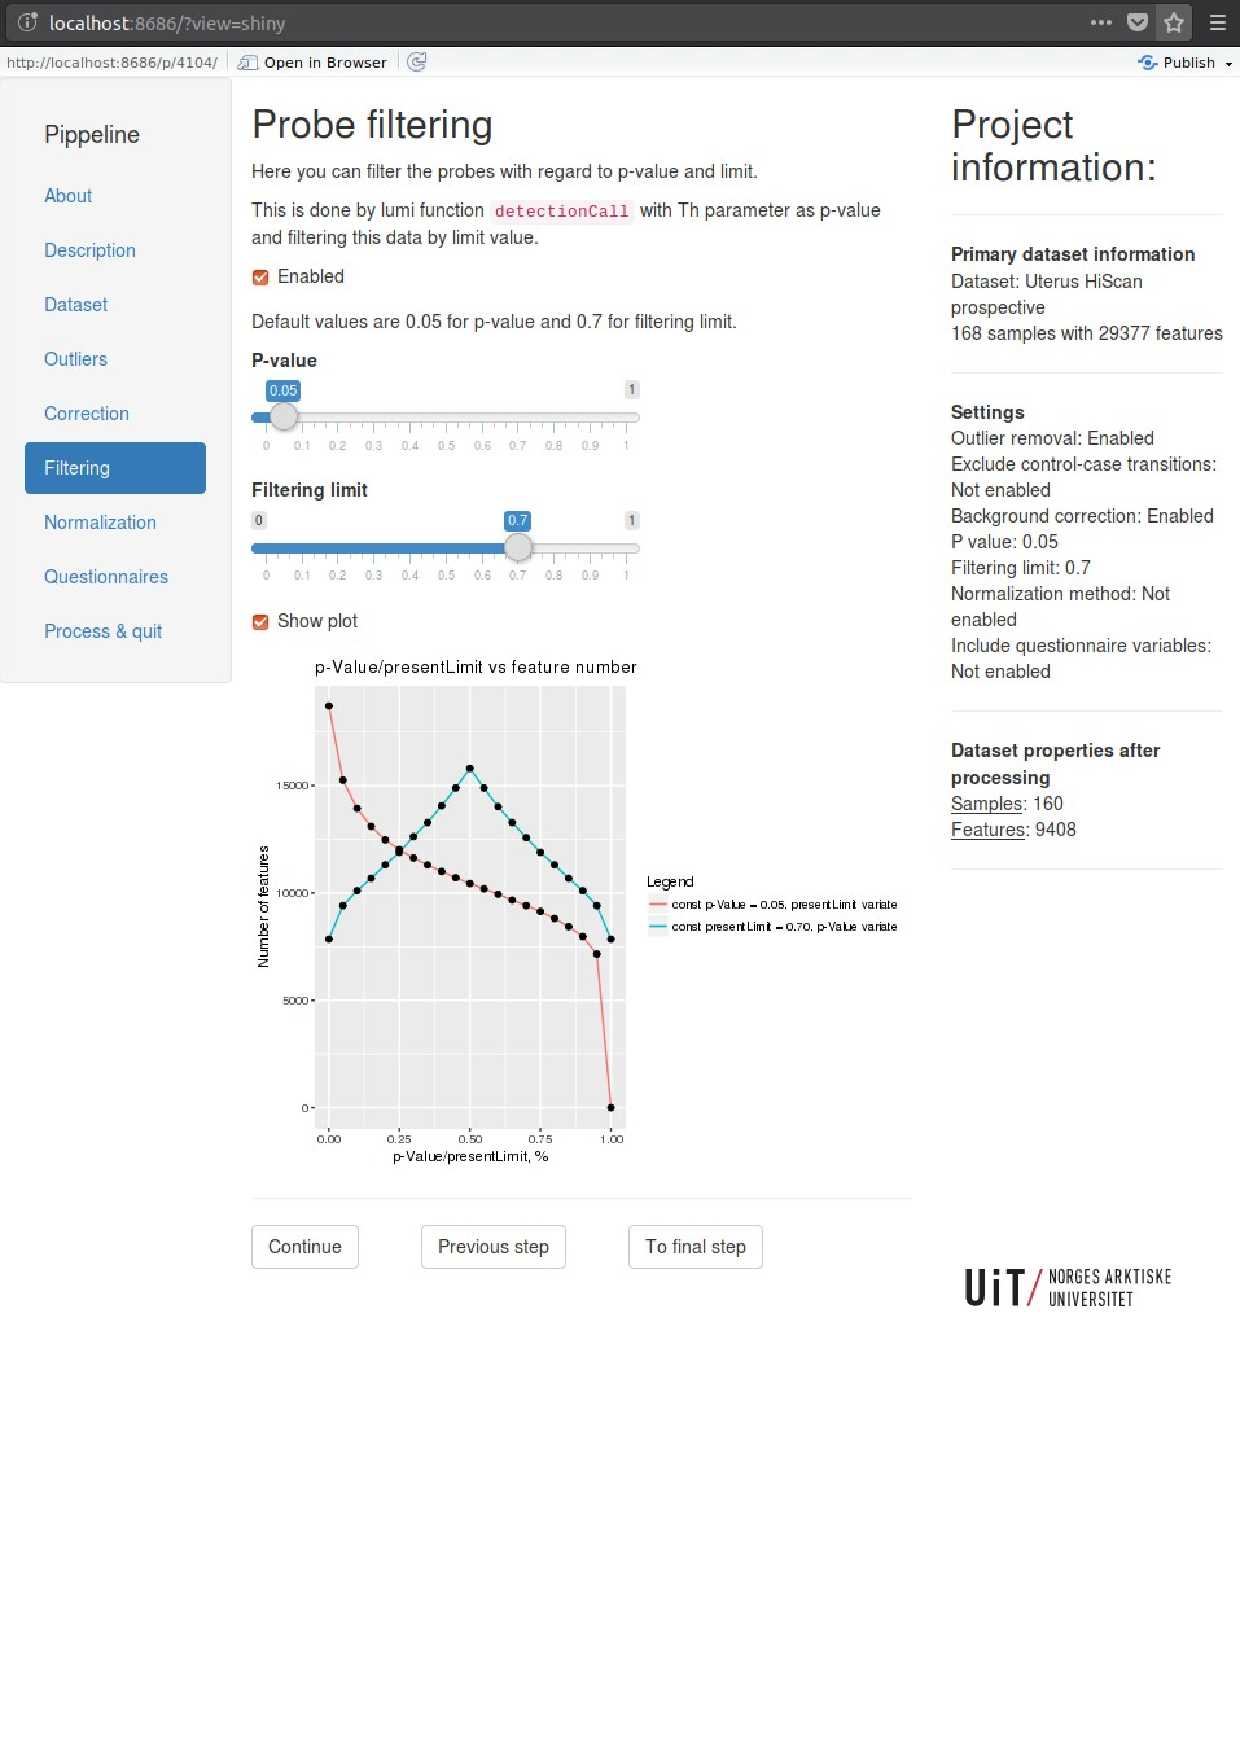
\includegraphics[width=\linewidth]{figures/scr_filtering.pdf}
    \caption[A screenshot of the web-interface of Pippeline.]{A screenshot of
    the web-interface of Pippeline. In the screenshot users can define at what
    level they want to filter out probes in the gene expression dataset. Users
    can define that the output dataset will only include gene expression probes
    that are present in a percent of the observation.}
  \label{fig:scr_filtering}
\end{figure}

\section{Best Practices} 
From our experiences we have developed a set of best practices for data
analysis. These apply both to researchers, and developers and the technical
staff managing the data in a research study: 

\textbf{Document every step in the analysis}. Analysis of modern datasets is a
complex exercise with the possibility of introducing an error in every step.
Analysts often use different tools and systems that require a particular set of
input parameters to produce results. Thoroughly document every step from raw
data to the final tables that go into a manuscript.

In the \gls{nowac} study we write help pages and reports for all datasets, and
the optional pre-processing steps. 

\textbf{Generate reports and papers using code}. With tools such as R
Markdown\cite{rmarkdown} and kntir there are few reasons for decoupling analysis
code with the presentation of the results through reports or scientific papers.
Doing so ensures the correctness reported results from the analyses, and greatly
simplifies reproducing the results in a scientific paper. 

In the \gls{nowac} study we produce reports from R code. These include
pre-processing and data delivery of datasets to researchers. One example of a
report is the analyses done in \cite{kiselev2018transcription} where we
documented the association between PAX6 gene expression and PAX6 target genes.
Through a simple R script we could share the results and underlying analysses.

\textbf{Version control everything}. Both code and data changes over the course
of a research project. Version control everything to make it possible to retrace
changes and the person responsible for them. It is often necessary to roll back
to previous versions or a dataset or analysis code, or to identify the
researches that worked on specific analyses. 

In the \gls{nowac} study we promote the use of git to version control both
source code and data. 

\textbf{Collaborate and share code through \gls{scm} systems}. Traditional
communication through e-mail makes it difficult to keep track of existing
analyses and their design choices both for existing project members and new
researchers. With \gls{scm} hosting systems such as Github developing
analysis code becomes more transparent to other collaborators, and encourages
collaboration. It also simplifies the process or archiving development decisions
such as choosing a normalization method.

In the \gls{nowac} study we collaborate on data analysis through a self-hosted
Gitlab\cite{gitlab} installation. We also open-source code on Github. 
% We have made our \texttt{nowac} R package and Pippeline online at
% \url{github.com/uit-bdps/nowac} and \url{github.com/uit-bdps/pippeline}. These
% public repositories do not contain any data, but analysis code and
% documentation. 
While we aim to make all our code, documentation, and datasets public, we are
unfortunately not there yet. We are working on a public version of the
\texttt{nowac} R package and the Pippeline, but we must guarantee that the
respective repositories do not contain any sensitive information from the
datasets. This is ongoing work. 

\section{Discussion}
In this chapter we have proposed an approach to enable reproducible analyses in
a complex epidemiological study. While we applied our approach to specific
research study, we believe that it is generalizable to other scientific
disciplines. 

We developed an R package for researchers in our study to simplify their
computational analyses. With the R package researchers could investigate the
available datasets and analyze them in the same environment. Providing a single
software package shortens the time to analysis, and improves researcher
productivity since they do not have to start from scratch when analyzing a new
dataset. In addition, it standardizes the analyses and makes the data analysis
process more transparent. We believe that our solution can be applied to
other datasets and projects within different scientific disciplines, enabling
more researchers to take advantage of the many collected, but not yet
analysis-ready datasets. 

Making science reproducible is of growing interest. In this chapter we outlined
the main best practices from our experiences in systems epidemiology research,
and believe that these are generalizable to other fields as well. The best
practices we arrived at follow the lines of other have described before
us,\cite{sandve2013ten} and we believe that these are necessary for both our
research group, but also to the scientific community, to follow. 

While taking advantage of powerful computational tools is beneficial, they often
require trained users.  A potential drawback of using an R package version
controlled in \texttt{git} to manage, document, and analyze research datasets is
the prerequisite programming skills for researchers. This may be an obstacle for
many researchers, but once they master the skills needed to analyze their data
programmatically, not just through a point-and-click interface, we believe that
it provides deeper knowledge into the analyses. While programming skills may be
absent in the training of many researchers, we believe that it is just a matter
of time before programming skills are common in the scientific community. 

While the majority of the researchers that have worked on the project have used
SAS for their analyses of the questionnaire data, all researchers working on
molecular data are using R. The great strength of R comes from its many
packages for analyzing, plotting, and interpreting data. An R package consists
of a code, documentation, tests, and data.  Bioconductor\cite{bioconductor} and
the \gls{cran}\cite{cran} provide online hosing for many packages, and users can
mix and match these packages to fit their need. 

There are many approaches to store and analyze biological datasets. Our approach
is targeted towards R users by building an R package, but as we demonstrate in
the next chapters, we have designed systems that interface directly with data
and analyses from outside the R ecosystem. 

One major drawback with the implementation of our approach in the \texttt{nowac}
R package is its size. While microarray datasets are relatively small compared
to sequencing data, when these datasets grow in number the total size grows as
well. This will impact the compile time for the R package, and also its size
when it is shared with other researchers. With larger datasets we might
experiment with extensions to git, e.g. \texttt{git-lfs} as we have done in
Chapter \ref{pipeline}.

Since we developed the Pippeline to preprocess our gene expression datasets, it
has been expanded to now work with RNA-seq, Methylation and microRNA datasets as
well. By using the Pippeline with new datasets researchers now have access to
the full preprocessing history behind each dataset available in the research
study. 

% GDPR & NOWAC, anything w/ a LPNR is sensitive 

\section{Conclusion}
In summary, we believe that there are four general rules toward reproducible
analyses. We believe that they apply to both our research study and other
similar epidemiological 
studies:
\begin{itemize} 
    \item Document and version control datasets and analysis code within the
        study. 
    \item Share datasets and analysis code through statistical software
        packages. 
    \item Share and report findings through reproducible data analysis reports. 
    \item Standardize and document common data preprocessing and wrangling
        steps.
\end{itemize} 

In this chapter we have demonstrated one approach that we believe help
researchers follow these to enable reproducible research. 

